\documentclass[12pt,a4paper]{article}
\usepackage[utf8]{inputenc}
\usepackage[english]{babel}
\usepackage[T1]{fontenc}
\usepackage{amsmath}
\usepackage{amsfonts}
\usepackage{amssymb}
\usepackage{graphicx}
\usepackage{verbatim}
\usepackage[left=2cm,right=2cm,top=2cm,bottom=2cm]{geometry}
\usepackage{siunitx}
\usepackage{placeins}
\usepackage{physics}
\author{Tim}
\usepackage{gensymb}
\usepackage{mathtools}
\usepackage{physics}
\begin{document}
\sisetup{separate-uncertainty = true}
	\setlength{\parindent}{0pt} 
	\begin{center}
		{\LARGE Exam}\\
		\begin{large}
			Computational Physics\\[0.4cm]
			Prof. Michielsen, Prof. Mazzarello\\[5.5cm]
			\Large\textbf{\textsl{Exercise 2: Orbit of a comet}}\\[5.5cm]
			\normalsize\textit{authored\\by}\\[0.4cm]
			\large\textbf{Moritz Berger (355244)\\moritz.berger@rwth-aachen.de}\\[2cm]
			\large{23.07.2019}
		\end{large}
	\end{center}
	\newpage
	
\section{Introduction}
In this exercise we want to simulate the orbit of a comet around the sun with the adaptive Runge-Kutta method. The equation of motion of this problem is
\begin{equation}
\dfrac{d^2}{dt^2} \vec{r} = \dfrac{GM}{|\vec{r}|^3} \vec{r}
\end{equation}
where we assume that the mass of the comet is much smaller than the mass of the sun and can be neglected. We use AU as unit of length and YR as unit of time which allows us to express $GM = 4 \pi^2 \si{AU^3/YR^2}$.\\
The goal of this exercise is to simulate the orbit of a comet starting \SI{1}{AU} away from the sun with different starting velocities and to determine the numerical eccentricity of the orbits. Furthermore the period $T$ and semi-major axis $a$ of these orbits are compared to Keplers third law.

\section{Simulation Model and Method}
The problem is simulated in a 2D-plane with the sun at position (0,0). The comet starts at position (1,0) with a velocity of $v = \pi/2, \pi, 2 \pi$ in (0,1) direction.\\
The problem is simulated using the adaptive 4th order Runge-Kutta method. From the equation of motion follows that the acceleration
$$ \vec{a} = \dfrac{-4 \pi^2}{|\vec{r}|^3} \vec{r}$$
is only dependent on the position $\vec r(t)$.

The method allows the calculation of the position and velocity after a time step $\tau$ by:
$$ r(t+\tau) = r(t) + \dfrac{1}{6} (k_1 + 2 k_2 + 2 k_3 + k_4)$$
$$ v(t+\tau) = v(t) + \dfrac{1}{6} (k_1' + 2 k_2' + 2 k_3' + k_4')$$
with the following Runge-Kutta terms:
$$ k_1 = \tau v(t) $$
$$ k_1' = \tau a(t) $$
$$ k_2 = \tau (v(t) + k_1'/2) $$
$$ k_2' = \tau a(r(t) + k_1/2) $$
$$ k_3 = \tau (v(t)+ k_2'/2) $$
$$ k_3' = \tau a(r(t) + k_2/2) $$
$$ k_4 = \tau (v(t)+ k_3') $$
$$ k_4' = \tau a(r(t) + k_3) $$

After calculation the local error of the position and velocity are checked. This is done by calculating two time steps of length $\tau/2$ and comparing the result with the one from the calculation with $\tau$:
$$ \epsilon_r' = |r(t+\tau) - r(t+\tau/2+\tau/2)|$$
$$ \epsilon_v' = |v(t+\tau) - v(t+\tau/2+\tau/2)|$$
if both errors are smaller than the error threshold $\sigma$, then the solution is accepted and the calculation continues with $t \rightarrow t+\tau$. If one of the errors is larger then the solution is rejected and the calculation starts again for the same time $t$. In both cases a new time step $\tau_{new}$ is defined by introducing the safety constants $S_1$ and $S_2$ and defining:
$$ \tau' = \left(\dfrac{\sigma}{\epsilon'}\right)^{1/5} \tau$$
$\epsilon'$ is here the larger one of the two errors in r and v.
The new time step is then given by:
\begin{equation*}
  \tau_{new} = \begin{cases}
        S_1 \tau' &\text{if $\tau/s_2 < S_1 \tau' < S_2 \tau$,} \\
        S_2 \tau &\text{if $S_1 \tau' > S_2 \tau$,} \\
        \tau/S_2 &\text{if $\tau/s_2 > S_1 \tau'$} \\
        \end{cases}
 \end{equation*}
The simulation is stopped after a full period or if the iterations exceed $m = 10000$.\\
For the simulation an initial time step of $\tau = 0.1$, $S_1 = 0.9$, $S_2 = 1.3$ and $\sigma = 10^{-10}$ are used. The suggested value of $\sigma = 10^{-3}$ resulted in very large steps at the aphelion (see appendix), which made the calculation of the period very inaccurate.\\

The eccentricity of the orbit is calculated by calculating the aphelion $r_a$ and perihelion $r_p$ and using the following formula:
\begin{equation}
\dfrac{r_a - r_p}{r_a + r_p}
\end{equation}
The semi-major axis is calculated by
$$\dfrac{r_a + r_p}{2}$$

\section{Results and Discussion}
\begin{table}[h]
\centering
\begin{tabular}{|c|c|c|c|c|}
\hline 
$v_0$[AU/YR] & $\epsilon$ & $\epsilon_{analytical}$ & $a$[AU] & $T$[YR] \\ 
\hline 
$\pi/2$ & 0.9375 & 0.9375 & 0.5161 & 0.3711\\
\hline 
$\pi$ & 0.7500 & 0.75 &0.5714 &0.4338\\ 
\hline 
$2\pi$ & $\SI{2e-9}{}$ & 0 & 1.0000 & 1.0000\\ 
\hline 
\end{tabular} 
\caption{Eccentricity, semi-major axis and period of the simulated orbits.}
\label{tab:Sandwich_Results}
\end{table}

The simulation is run for three different starting velocities. The results are shown in figure \ref{fig:results}. The eccentricity can also be calculated analytically:
$$\epsilon = \sqrt{1+\dfrac{2 E h^2}{(GM)^2}}$$
with the specific energy $E = v^2/2 - GM/r$ and the specific angular momentum $h = v_0$.\\
All calculated orbital parameters can be found in table \ref{tab:Sandwich_Results}. The eccentricity of the simulated orbits agree with the analytical results.\\

In figure \ref{fig:kepler} $a^3$ is plotted against $T^2$. According to Keplers 3rd law the following holds true for all orbits in a system:
\begin{equation*}
\dfrac{a_1^3}{T_1^2} = \dfrac{a_2^3}{T_2^2} = \dfrac{a_3^3}{T_3^2} = \SI{1}{AU^3/YR^2}
\end{equation*}
This means that the points in figure \ref{fig:kepler} should be on a line with a slope of 1, which is the case. The simulated orbits therefore fulfill Keplers 3rd law.

\begin{figure}
\centering
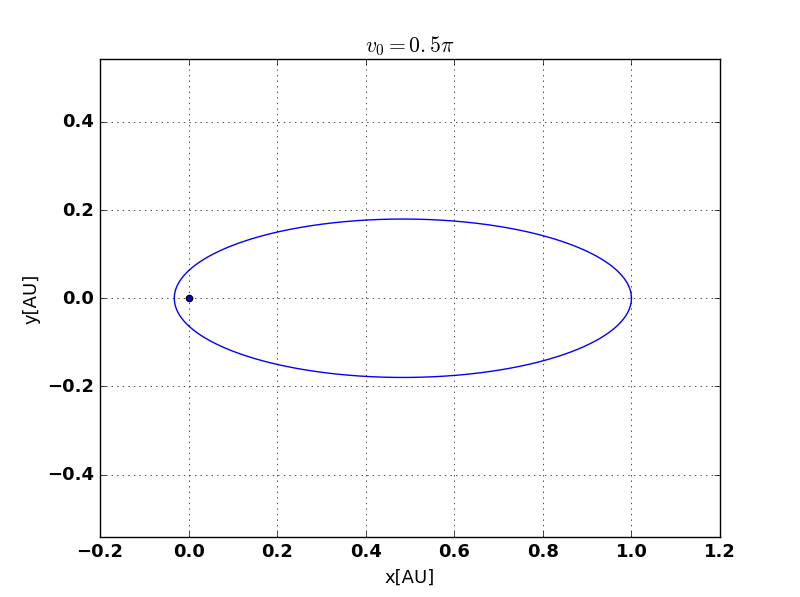
\includegraphics[scale=0.5]{Bilder/05.png}
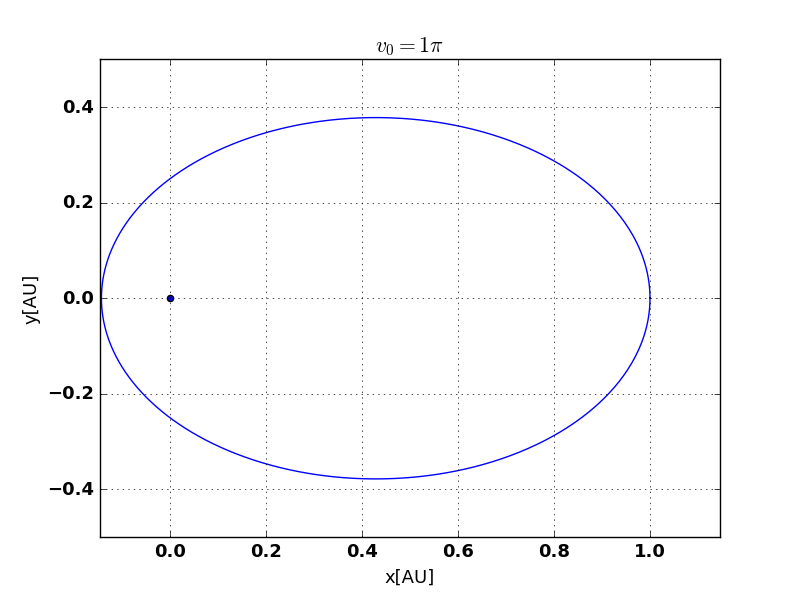
\includegraphics[scale=0.5]{Bilder/1.png}
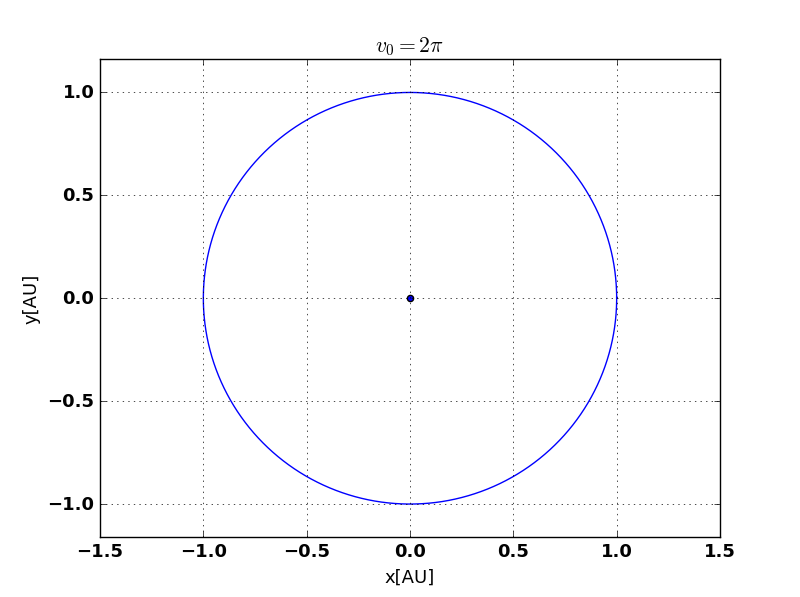
\includegraphics[scale=0.5]{Bilder/2.png}
\caption{Orbital trajectory for $v = \pi/2, \pi, 2 \pi$ and starting position (1,0). The position of the sun is marked with a dot.}
\label{fig:results}
\end{figure}

\begin{figure}
\centering
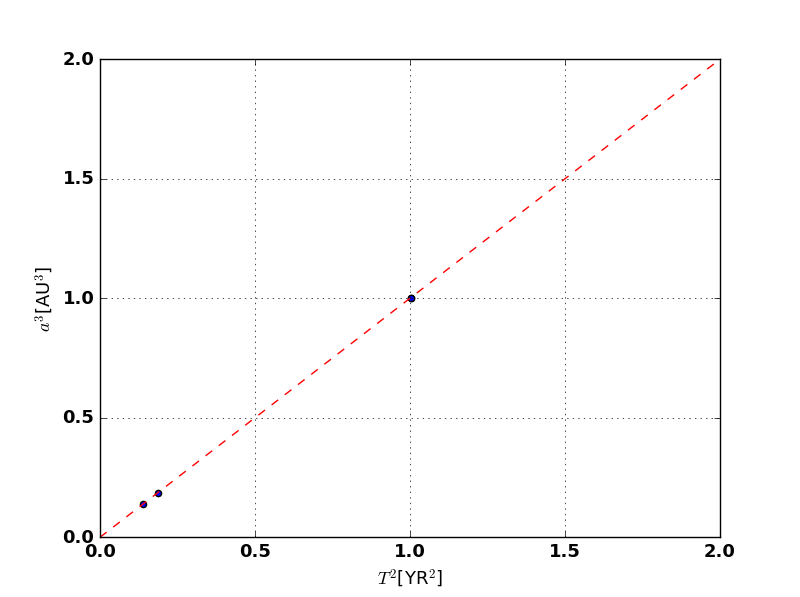
\includegraphics[scale=0.5]{Bilder/kepler.png}
\caption{Third power of the semi-major axis plotted against the second power of the period. The red line indicates Keplers 3rd law.}
\label{fig:kepler}
\end{figure}
\newpage
\section{Appendix}
\begin{figure}[h]
\centering
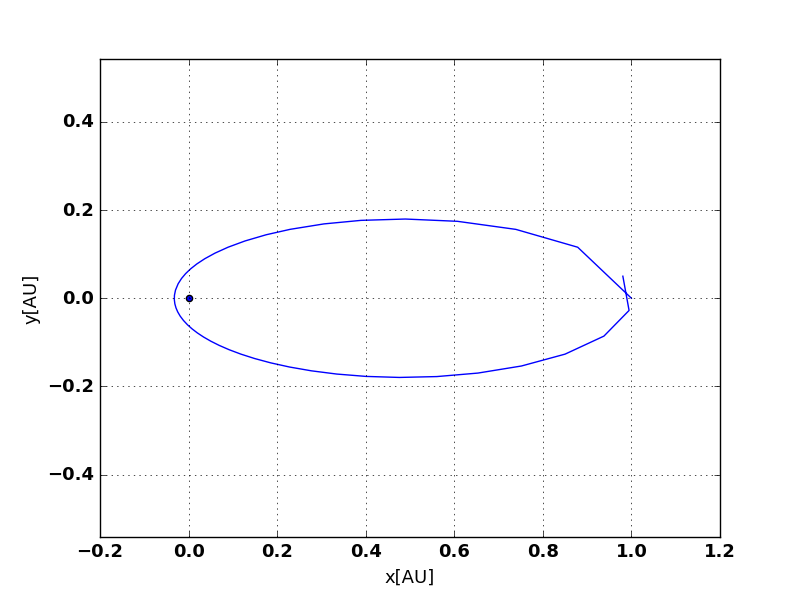
\includegraphics[scale=0.5]{Bilder/appendix.png}
\caption{Orbital trajectory for $v = \pi/2$ calculated with an error threshold of $\sigma = 0.001$. The steps at the aphelion are very large, making the determination of the orbital period inaccurate.}
\label{fig:app}
\end{figure}
\end{document}



\